\providecommand{\main}{..} %Important: It needs to be defined before the documentclass

\documentclass[\main/main.tex]{subfiles}

\begin{document}

\subsection{The Perron–Frobenius theorem}
The Perron–Frobenius theorem is a set of results about eigenvalues of nonnegative matrices. Recall that a matrix is \lq\lq \textit{nonnegative} if all its elements are $\geq 0$'', and \lq\lq \textit{positive} if all its elements are strictly $> 0$" \citep{Keyfitz2005}. 

In order to understand the main results of this theorem, first of all one needs to consider the following classification of nonnegative matrices \citep{Keyfitz2005} 


\begin{figure}[h!]
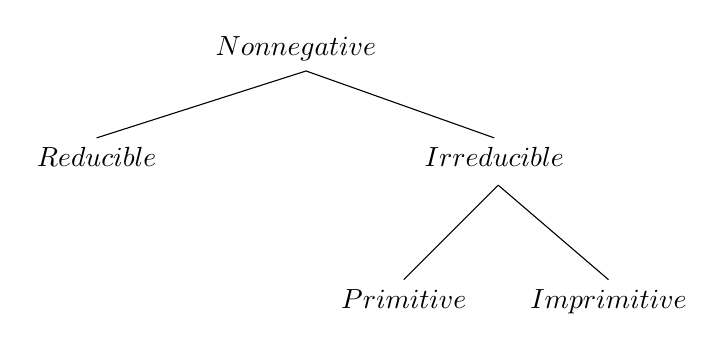
\begin{tikzpicture}[scale=1]
\draw (3.83, 2.65) node [above] {$Nonnegative$};
\draw (3.96, 2.65) -- (6.35, 1.8) node [below] {$Irreducible$};
\draw (3.96, 2.65) -- (1.3, 1.8) node [below] {$Reducible$};
\draw (6.4, 1.2) -- (5.2, 0) node [below] {$Primitive$};
\draw (6.4, 1.2) -- (7.8, 0) node [below] {$Imprimitive$};
\end{tikzpicture}
\caption{Properties of nonnegative matrices}
\end{figure}

Nonnegative matrices can be divided into \lq\lq reducible and irreducible matrices; irreducible matrices in turn are divided into primitive and imprimitive matrices'' \citep{Keyfitz2005}.

\subsubsection{Notation and definitions}

A \textit{path} from $s_i$ to $s_j$ is a sequence of steps that begins at $s_i$ and ends at $s_j$, passing through no node more than once, in the direction indicated by the arrows in a transition diagram.\\
A \textit{loop} is a path from a node to itself.\\
The \textit{length} of a path or a loop is the number of steps it contains. A self-loop has length 1. For instance, the sequence $s_1 \rightarrow s_2  \rightarrow s_3$ is a path of length 2 from $s_1$ to $s_3$ . The sequence $s_1 \rightarrow s_2 \rightarrow s_1 \rightarrow s_2  \rightarrow s_3$ is not a path, because it passes through $s_2 $ twice.\\
A nonnegative matrix is \textit{irreducible} \lq\lq if and only if its life cycle graph contains a path from every node to every other node'' \citep{Keyfitz2005}. In other words, the life cycle graph is \lq\lq strongly connected'', i.e. every node is reachable from any other node of the graph. Conversely, if some stages do not contribute to other stages of the life cycle, the nonnegative is said to be \textit{reducible}.
Irreducible matrices can in turn be divided into \textit{primitive} and \textit{imprimitive} ones. 
If, raising a matrix to sufficiently high powers, allows the matrix 


An irreducible nonnegative matrix is primitive if it becomes positive when raised to sufficiently high powers'' \citep{Keyfitz2005}, i.e., if Ak is strictly positive for some k> 0. A reducible matrix cannot be primitive, because when the matrix in (7.2.1) is raised to powers, the upper-right block remains zero. Primitivity



Equation \ref{eq:1} has an analytical solution that is based on the concepts of eigenvalues and eigenvectors. What follows is taken from \cite{Keyfitz2005}.

\noindent \textit{Eigenvectors and eigenvalues.} A vector \textbf{w} is said to be a right eigenvector of the matrix \textbf{A} and the scalar $\lambda$ is said to be the corresponding eigenvalue if the following is satisfied:
\begin{equation} \label{eq:2}
    \mathbf{Aw} = \lambda \mathbf{w}
\end{equation}
which implies that
\begin{equation} \label{eq:2}
    (\mathbf{A} - \lambda \mathbf{I}) \mathbf{w} =\mathbf{0} 
\end{equation}
where $\mathbf{I}$ is the identity matrix and $\mathbf{0} $ is a vector of 0. 
$\mathbf{w}$ has a non-zero solution only if $(\mathbf{A} - \lambda \mathbf{I})$ is singular, i.e. its determinant is equal to zero:
\begin{equation}\label{eq:3}
    det (\mathbf{A} - \lambda \mathbf{I}) = 0
\end{equation}
Equation \ref{eq:3} is called the characteristic equation.\
If the matrix $\mathbf{A}$ has dimension $s \times s$ it follows that the characteristic equation will be a polynomial of sth-order, the matrix $\mathbf{A}$ will have $s$ eigenvalue-eigenvectors pairs, and each pair will be a solution to the characteristic equation. In the derivation proposed by \cite{Keyfitz2005}, the eigenvectors are assumed to be linearly independent.

\noindent \textit{Derivation.} Start with writing the initial population $\mathbf{n}_0$ as a linear combination of the right eigenvectors $w_i$ of $\mathbf{A}$:

\begin{equation}
\begin{split}
    \mathbf{n}_0 &= c_1 \mathbf{w_1} + c_2 \mathbf{w_2} + ... + c_s \mathbf{w_s} = \\
    &= (\mathbf{w_1} \; \cdots \; \mathbf{w_s})
\begin{pmatrix}
c_1 \\ \vdots \\c_s
\end{pmatrix}  =\\
&= \mathbf{Wc}\\
\end{split}
\end{equation}
where $\mathbf{W}$ is a matrix whose columns are the all the eigenvectors $w_i$ while $ \mathbf{c}$ is a column vector containing the $c_i$ coefficients.

If we multiply $\mathbf{n}_0$ by $\mathbf{A}$:
\begin{equation}
    \mathbf{A} \mathbf{n}_0 = \mathbf{A} \mathbf{Wc} = \mathbf{A}  \sum_{i} w_i
\end{equation}





The main ideas were already explored by \cite{Feichtinger1973} in the 1970's.




Markov Chain models belong to the broader framework of matrix population models. In the following section, I will review the main concepts of the general framework and then focus on the transition matrix of the Markov Chain.

\subsection{Matrix Population Models}

Markov chain are described by the so-called a \lq\lq stochastic matrix'' or a \lq\lq Markov matrix'', a matrix used to describe the probabilities of the possible transitions in a process .

A Matrix Population Model can be used to project population growth:

\begin{equation}\label{eq:1}
    \mathbf{n} (t+1) = \mathbf{An}(t)
\end{equation}
where $\mathbf{n} (t+1)$ is a population vector representing the number of individuals in each subgroup at time $t +1$ (e.g. the age classes in which we have decided to categorised the population), $\mathbf{A}$ is the stage or age-classified projection matrix, and $\mathbf{n} (t)$ is the population vector at time $t$, also called the vector of abundances of the stages.
Each entry $a_{ij}$ of the matrix $\mathbf{A}$ represents the expected number of individuals in stage $i$ at time $t + 1$ that at time $t$ were at stage $j$. 

Typically, the matrix $\mathbf{A}$ is partioned into a matrix $\mathbf{U}$, which describes the transitions of surviving individuals from time $t$ to $t+1$, and into a matrix $\mathbf{F}$, representing fertility:
\begin{equation}
    \mathbf{A} =  \mathbf{U} + \mathbf{F}
\end{equation}

The life cycle stages can be transient (e.g. the subsequent age classes) or absorbing (e.g. death). Note that the matrix $\mathbf{U}$ represents only the transient stages of surviving individuals.
When death is takes into consideration, we describe the absorbing Markov chain with the matrix $\mathbf{P}$, constructed as follows:

\begin{equation}
    \mathbf{P} = \begin{pmatrix}
        \mathbf{U} &  0\\
    \mathbf{m}& 1
    \end{pmatrix}
\end{equation}
where $\mathbf{m}$ is a  $1 \times j$ vector describing the probability of dying for an individual in stage $j$.
This idea can be extended to the case in which different causes of death are considered:
\begin{equation}
    \mathbf{P} = \begin{pmatrix}
        \mathbf{U} &  0\\
    \mathbf{M}& 1
    \end{pmatrix}
\end{equation}
by replacing the vector $\mathbf{m}$ with the matrix $\mathbf{M}$.

The transition matrix $\mathbf{P}$ is called \lq\lq Each of its entries is a nonnegative real number representing a probability.[column-stochastic

Equation \ref{eq:1} has an analytical solution that is based on the concepts of eigenvalues and eigenvectors. What follows is taken from \cite{Keyfitz2005}.

\noindent \textit{Eigenvectors and eigenvalues.} A vector \textbf{w} is said to be a right eigenvector of the matrix \textbf{A} and the scalar $\lambda$ is said to be the corresponding eigenvalue if the following is satisfied:
\begin{equation} \label{eq:2}
    \mathbf{Aw} = \lambda \mathbf{w}
\end{equation}
which implies that
\begin{equation} \label{eq:2}
    (\mathbf{A} - \lambda \mathbf{I}) \mathbf{w} =\mathbf{0} 
\end{equation}
where $\mathbf{I}$ is the identity matrix and $\mathbf{0} $ is a vector of 0. 
$\mathbf{w}$ has a non-zero solution only if $(\mathbf{A} - \lambda \mathbf{I})$ is singular, i.e. its determinant is equal to zero:
\begin{equation}\label{eq:3}
    det (\mathbf{A} - \lambda \mathbf{I}) = 0
\end{equation}
Equation \ref{eq:3} is called the characteristic equation.\
If the matrix $\mathbf{A}$ has dimension $s \times s$ it follows that the characteristic equation will be a polynomial of sth-order, the matrix $\mathbf{A}$ will have $s$ eigenvalue-eigenvectors pairs, and each pair will be a solution to the characteristic equation. In the derivation proposed by \cite{Keyfitz2005}, the eigenvectors are assumed to be linearly independent.

\noindent \textit{Derivation.} Start with writing the initial population $\mathbf{n}_0$ as a linear combination of the right eigenvectors $w_i$ of $\mathbf{A}$:

\begin{equation}
\begin{split}
    \mathbf{n}_0 &= c_1 \mathbf{w_1} + c_2 \mathbf{w_2} + ... + c_s \mathbf{w_s} = \\
    &= (\mathbf{w_1} \; \cdots \; \mathbf{w_s})
\begin{pmatrix}
c_1 \\ \vdots \\c_s
\end{pmatrix}  =\\
&= \mathbf{Wc}\\
\end{split}
\end{equation}
where $\mathbf{W}$ is a matrix whose columns are the all the eigenvectors $w_i$ while $\mathbf{c}$ is a column vector containing the $c_i$ coefficients.

If we multiply $\mathbf{n}_0$ by $\mathbf{A}$:
\begin{equation}
    \mathbf{A} \mathbf{n}_0 = \mathbf{A} \mathbf{Wc} = \mathbf{A}  \sum_{i} w_i
\end{equation}


\end{document}